% Provenance (never printed): see sources/outline_sources.md (Year 1: optical
% mineralogy with the polarising microscope; Michel-Levy chart). Interference
% colours in figdata/bachelor-1/michel_levy.py from the CIE 1931 colour-matching
% functions and illuminant D65 (data/derived/bachelor-1-cie*.csv); exercise and
% problem values in the Book 3 scratch calculator calc/ch08.py.
\chapter{Optical Mineralogy}\label{ch:b1:optical-mineralogy}

Between \omterm{def:b1:field-lab-methods-1:microscope}{crossed polars} a \omterm{def:b1:field-lab-methods-1:thin-section}{thin section} of gabbro lights up like stained glass.
Long grey and white laths, striped like a barcode, cross the field; between
them, grains glow blue, yellow and magenta; a few stay black whatever the
angle. Each of these effects has a cause that can be calculated, and each
tells which \omterm{def:b1:rock-forming-minerals:mineral}{mineral} is there. This chapter explains how light crosses a
crystal, why a \omterm{def:b1:rock-forming-minerals:mineral}{mineral} between \omterm{def:b1:field-lab-methods-1:microscope}{crossed polars} is coloured, how the colour
measures a property of the \omterm{def:b1:rock-forming-minerals:mineral}{mineral}, and how a petrologist names the grains of
a \omterm{def:b1:field-lab-methods-1:thin-section}{thin section} with nothing but a microscope. It ends with an unknown section
whose \omterm{def:b1:rock-forming-minerals:mineral}{minerals}, and whose \omterm{def:b1:cross-sections:thickness}{true thickness}, are found from what it shows.

\begin{recall}
A \omterm{def:b1:field-lab-methods-1:thin-section}{thin section} is a slice of rock about \qty{30}{\micro m} thick on a glass
slide; the \omterm{def:b1:field-lab-methods-1:microscope}{polarising microscope} looks at it in \omterm{def:b1:field-lab-methods-1:microscope}{plane-polarised light} (one
polariser) and between \omterm{def:b1:field-lab-methods-1:microscope}{crossed polars} (\cref{ch:b1:field-lab-methods-1}). The
refractive index $n$ of a medium is the ratio of the speed of light in vacuum
to its speed in the medium, and refraction at an interface obeys Snell's law
$n_1\sin i_1 = n_2\sin i_2$ (physics, University Year 1). Light is a
transverse wave; a polariser passes only the component of the electric field
along its direction, so that an analyser at angle $\alpha$ to it passes the
fraction $\cos^2\alpha$ of the intensity (Malus's law, physics).
\end{recall}

\section{Light in crystals}

In a glass, a liquid or a cubic crystal, light travels at the same speed in
every direction and whatever its vibration direction. In most \omterm{def:b1:rock-forming-minerals:mineral}{minerals} it
does not: the arrangement of atoms differs along different directions, and so
does the response of the electrons to the electric field of the wave.

\begin{definition}[Isotropic and anisotropic minerals]\label{def:b1:optical-mineralogy:anisotropic}
A \omterm{def:b1:rock-forming-minerals:mineral}{mineral} is an \emph{isotropic mineral}\index{isotropic mineral} when its
refractive index is the same for every direction of propagation and of
vibration of light; cubic \omterm{def:b1:rock-forming-minerals:mineral}{minerals} (\omterm{def:b1:rock-forming-minerals:groups}{garnet}, halite, spinel) and glasses are
isotropic. It is an \emph{anisotropic mineral}\index{anisotropic mineral}
when its refractive index depends on the vibration direction; all \omterm{def:b1:rock-forming-minerals:mineral}{minerals}
of the other crystal systems are anisotropic.
\end{definition}

A plate cut from an anisotropic crystal does not let light through as a single
wave. We admit the following result of crystal optics (physics, University
Year 2): for a given direction of propagation, a plate of an \omterm{def:b1:optical-mineralogy:anisotropic}{anisotropic
mineral} transmits two waves that vibrate in two perpendicular directions fixed
in the plate, its \emph{vibration directions}, and travel with two different
refractive indices $n_1$ and $n_2$. Light vibrating along one of these
directions crosses the plate unchanged in polarisation; light vibrating in any
other direction is split into its two components along them. The two indices
depend on the direction of propagation, and there are particular directions
in which they are equal.

\begin{definition}[Optic axis, uniaxial and biaxial minerals]\label{def:b1:optical-mineralogy:optic-axis}
An \emph{optic axis}\index{optic axis} of an \omterm{def:b1:optical-mineralogy:anisotropic}{anisotropic mineral} is a
direction of propagation along which light travels with a single refractive
index, whatever its vibration direction, as in an isotropic medium. A \omterm{def:b1:rock-forming-minerals:mineral}{mineral}
is \emph{uniaxial}\index{uniaxial} when it has one optic axis (\omterm{def:b1:rock-forming-minerals:mineral}{minerals} of the
trigonal, tetragonal and hexagonal systems, such as quartz and calcite) and
\emph{biaxial}\index{biaxial} when it has two (orthorhombic, monoclinic and
triclinic \omterm{def:b1:rock-forming-minerals:mineral}{minerals}, such as \omterm{def:b1:rock-forming-minerals:groups}{olivine}, \omterm{def:b1:rock-forming-minerals:groups}{pyroxenes}, \omterm{def:b1:rock-forming-minerals:groups}{amphiboles}, \omterm{def:b1:rock-forming-minerals:groups}{micas} and
\omterm{def:b1:rock-forming-minerals:groups}{feldspars}).
\end{definition}

The geometry is summarised by a surface, the indicatrix: an ellipsoid whose
radius in each direction is the refractive index for light vibrating in that
direction. The section of the ellipsoid perpendicular to the direction of
propagation is an ellipse whose axes are the two vibration directions and
whose semi-axes are $n_1$ and $n_2$. For a \omterm{def:b1:optical-mineralogy:optic-axis}{uniaxial} \omterm{def:b1:rock-forming-minerals:mineral}{mineral} the ellipsoid is
one of revolution about the \omterm{def:b1:optical-mineralogy:optic-axis}{optic axis}, with two principal indices $n_\omega$
and $n_\varepsilon$: quartz has $n_\omega = 1.544$ and $n_\varepsilon = 1.553$,
calcite $1.658$ and $1.486$.
% ledger: hom:quartz-optics, hom:calcite-optics
A \omterm{def:b1:optical-mineralogy:optic-axis}{biaxial} \omterm{def:b1:rock-forming-minerals:mineral}{mineral} has three principal indices $n_\alpha < n_\beta < n_\gamma$
and two circular sections, perpendicular to its two optic axes: forsterite has
$1.635$, $1.651$ and $1.670$.
% ledger: hom:forsterite-optics

\begin{definition}[Birefringence (of a mineral)]\label{def:b1:optical-mineralogy:birefringence}
The \emph{birefringence}\index{birefringence (of a mineral)} of a \omterm{def:b1:rock-forming-minerals:mineral}{mineral} is
the difference $\delta = n_{\max} - n_{\min}$ between its largest and its
smallest principal refractive indices: $n_\varepsilon - n_\omega$ in absolute
value for a \omterm{def:b1:optical-mineralogy:optic-axis}{uniaxial} \omterm{def:b1:rock-forming-minerals:mineral}{mineral}, $n_\gamma - n_\alpha$ for a \omterm{def:b1:optical-mineralogy:optic-axis}{biaxial} one. In a
grain cut in any other direction, the difference $|n_1 - n_2|$ lies between 0
(a section perpendicular to an \omterm{def:b1:optical-mineralogy:optic-axis}{optic axis}) and $\delta$ (a section containing
the directions of $n_{\max}$ and $n_{\min}$).
\end{definition}

The \omterm{def:b1:optical-mineralogy:birefringence}{birefringence} is a property of the \omterm{def:b1:rock-forming-minerals:mineral}{mineral}, like its density: quartz
\num{0.009}, calcite \num{0.172}, forsterite \num{0.035}, fayalite
\num{0.052}. A \omterm{def:b1:field-lab-methods-1:thin-section}{thin section} cuts the grains of a \omterm{def:b1:rock-forming-minerals:mineral}{mineral} in every
orientation, so its grains show every value from 0 to $\delta$; only the
highest is characteristic.
% ledger: hom:quartz-optics, hom:calcite-optics, hom:forsterite-optics, hom:fayalite-optics

\section{Observations in plane-polarised light}

With the lower polariser only, the microscope shows the shape of the grains,
their colour, their cleavages and their \omterm{def:b1:optical-mineralogy:relief}{relief}.

\begin{definition}[Pleochroism]\label{def:b1:optical-mineralogy:pleochroism}
A \omterm{def:b1:rock-forming-minerals:mineral}{mineral} is \emph{pleochroic}\index{pleochroism} when its colour, seen in
\omterm{def:b1:field-lab-methods-1:microscope}{plane-polarised light}, changes as the stage is rotated; the
\emph{pleochroism} is this change. It arises because the absorption of light
depends on its vibration direction in the crystal.
\end{definition}

Biotite is the textbook case: a grain cut across its cleavage passes from pale
yellow-brown to dark brown as it turns, darkest when the cleavage traces lie
along the polariser. Hornblende changes from yellow to green. Most other
rock-forming silicates (quartz, \omterm{def:b1:rock-forming-minerals:groups}{feldspars}, \omterm{def:b1:rock-forming-minerals:groups}{olivine}, diopside, muscovite) are
colourless in \omterm{def:b1:field-lab-methods-1:thin-section}{thin section}, and their colourless grains are told apart by
other means.
% ledger: hom:biotite-optics, hom:hornblende-optics, hom:muscovite-optics, hom:diopside-optics, hom:forsterite-optics

\begin{definition}[Relief, Becke line]\label{def:b1:optical-mineralogy:relief}
The \emph{relief}\index{relief (optical)} of a grain in \omterm{def:b1:field-lab-methods-1:thin-section}{thin section} is how
strongly its outline, cracks and surface stand out against the mounting
medium; it is high when the refractive indices of the grain and of the medium
differ much, low when they are close. The \emph{Becke line}\index{Becke line}
is the thin bright line that borders a grain whose index differs from that of
its surroundings when the microscope is slightly out of focus.
\end{definition}

\begin{proposition}[Relief and refractive index]\label{prop:b1:optical-mineralogy:relief}
A ray crossing at incidence $i$ a boundary between a mounting medium of index
$n_m$ and a grain of index $n$ close to $n_m$ is deviated by
\[
  \varepsilon \approx \frac{|n - n_m|}{n_m}\,\tan i
\]
(in radians), to first order in $(n - n_m)/n_m$. The deviations at the
inclined edges of a grain, and so its \omterm{def:b1:optical-mineralogy:relief}{relief}, grow in proportion to
$|n - n_m|$.
\end{proposition}

\begin{proof}
Snell's law gives $n_m \sin i = n \sin r$. Write $n = n_m(1 + \eta)$ with
$\eta$ small and $r = i - \varepsilon$ with $\varepsilon$ small. Then
$\sin i = (1 + \eta)(\sin i - \varepsilon\cos i) + O(\eta^2, \varepsilon^2)$,
so $\eta \sin i = \varepsilon\cos i$ to first order, that is
$\varepsilon = \eta\tan i$, with $|\eta| = |n - n_m|/n_m$.
\end{proof}

A \omterm{def:b1:field-lab-methods-1:thin-section}{thin section} is mounted in a resin of index about $1.54$.
% ledger: jaic:epoxy-ri
Quartz ($1.544$--$1.553$) and the \omterm{def:b1:rock-forming-minerals:groups}{feldspars} ($1.52$--$1.59$) are nearly
invisible against it: low \omterm{def:b1:optical-mineralogy:relief}{relief}, the grain boundaries hard to see. \omterm{def:b1:rock-forming-minerals:groups}{Olivine}
($1.64$--$1.88$), \omterm{def:b1:rock-forming-minerals:groups}{pyroxenes} and \omterm{def:b1:rock-forming-minerals:groups}{amphiboles} stand out with dark rims and a
rough-looking surface: high \omterm{def:b1:optical-mineralogy:relief}{relief}. \omterm{def:b1:rock-forming-minerals:groups}{Garnet} ($1.83$) looks almost black-rimmed.
Calcite, whose index runs from $1.486$ to $1.658$ with the vibration
direction, changes \omterm{def:b1:optical-mineralogy:relief}{relief} as the stage turns, an effect called twinkling.
% ledger: hom:quartz-optics, hom:albite-optics, hom:anorthite-optics, hom:orthoclase-optics, hom:forsterite-optics, hom:fayalite-optics, hom:almandine-optics, hom:calcite-optics
The \omterm{def:b1:optical-mineralogy:relief}{relief} tells only how far $n$ is from $n_m$, not on which side; the \omterm{def:b1:optical-mineralogy:relief}{Becke
line} tells the side.

\begin{method}[The Becke line test]\label{met:b1:optical-mineralogy:becke}
Focus on the edge of a grain in \omterm{def:b1:field-lab-methods-1:microscope}{plane-polarised light}, close the aperture
diaphragm a little, and raise the focus slightly (move the objective away from
the section). The bright \omterm{def:b1:optical-mineralogy:relief}{Becke line} moves into the medium of higher refractive
index: if it moves into the grain, the grain has the higher index (positive
\omterm{def:b1:optical-mineralogy:relief}{relief}); if it moves out into the mount or the neighbouring grain, the grain
has the lower index (negative \omterm{def:b1:optical-mineralogy:relief}{relief}).
\end{method}

The method works because a grain boundary is never exactly vertical: at an
inclined boundary, light is refracted towards the side of higher index, and
beyond the critical angle it is totally reflected on that side, so that the
light crossing the boundary is concentrated above the higher-index medium.
Raising the focus looks at a plane above the section, where that concentrated
light lies inside the higher-index material.

\section{Between crossed polars}

With the analyser inserted, at right angles to the polariser, an isotropic
grain is black in every position: light reaches it vibrating along the
polariser and leaves it vibrating the same way, and the analyser stops it
entirely. An anisotropic grain is generally bright and coloured. The reason
is the delay between its two waves.

\begin{definition}[Retardation (in a crystal plate)]\label{def:b1:optical-mineralogy:retardation}
The \emph{retardation}\index{retardation (in a crystal plate)} $\Delta$ of a
plate of an \omterm{def:b1:optical-mineralogy:anisotropic}{anisotropic mineral} is the difference between the optical paths of
its two waves on leaving the plate, the slower wave lagging behind the faster.
\end{definition}

\begin{proposition}[Retardation and birefringence]\label{prop:b1:optical-mineralogy:retardation}
A plate of thickness $d$ whose two waves have indices $n_1 > n_2$ has the
\omterm{def:b1:optical-mineralogy:retardation}{retardation}
\[
  \Delta = d\,(n_1 - n_2),
\]
and its two waves leave it with a phase difference $\varphi = 2\pi\Delta/\lambda$
for light of wavelength $\lambda$ in vacuum. In a \omterm{def:b1:field-lab-methods-1:thin-section}{thin section}, the
largest \omterm{def:b1:optical-mineralogy:retardation}{retardation} shown by grains of one \omterm{def:b1:rock-forming-minerals:mineral}{mineral} is $d\,\delta$.
\end{proposition}

\begin{proof}
A wave crossing a thickness $d$ at speed $c/n$ takes the time $nd/c$; its
optical path, the distance light would cover in vacuum in that time, is $nd$.
The two waves enter together; on leaving, the slower one is behind by
$n_1 d - n_2 d = d(n_1 - n_2)$, a delay that is the fraction $\Delta/\lambda$
of a period, that is a phase $2\pi\Delta/\lambda$. The largest value of
$n_1 - n_2$ among all orientations is $\delta$
(\cref{def:b1:optical-mineralogy:birefringence}).
\end{proof}

A quartz grain of the most favourable orientation in a section
\qty{30}{\micro m} thick has $\Delta = \qty{30000}{nm}\times0.009 =
\qty{270}{nm}$; a calcite grain $\qty{30000}{nm}\times0.172 = \qty{5160}{nm}$.

\begin{omfigure}
\begin{tikzpicture}[x=1cm, y=1cm, >={Stealth},
  sub/.style={align=center, font=\small, text width=4.2cm}]
% (a) the polariser
\begin{scope}
  \draw[gray!60] (-1.4,0) -- (1.4,0) (0,-1.4) -- (0,1.4);
  \node[gray, font=\scriptsize] at (1.55,-0.2) {E};
  \node[gray, font=\scriptsize] at (0.2,1.55) {N};
  \draw[very thick, omDef, <->] (-1.2,0) -- (1.2,0);
  \node[omDef, font=\scriptsize, above] at (0.75,0.05) {$E_0$};
  \node[sub] at (0,-2.1) {(a) after the polariser:\\ vibration east--west};
\end{scope}
% (b) inside the plate
\begin{scope}[shift={(5.0,0)}]
  \draw[gray!60] (-1.4,0) -- (1.4,0) (0,-1.4) -- (0,1.4);
  \draw[omThm, thick] (-1.35*0.866,-1.35*0.5) -- (1.35*0.866,1.35*0.5);
  \draw[omThm, thick] (1.35*0.5,-1.35*0.866) -- (-1.35*0.5,1.35*0.866);
  \node[omThm, font=\scriptsize] at (1.42,0.95) {1};
  \node[omThm, font=\scriptsize] at (-0.85,1.32) {2};
  \draw[very thick, omDef, ->] (0,0) -- (1.2,0);
  \draw[omProp, very thick, ->] (0,0) -- (1.2*0.866*0.866,1.2*0.866*0.5);
  \draw[omProp, very thick, ->] (0,0) -- (1.2*0.5*0.5,-1.2*0.5*0.866);
  \draw[densely dotted] (1.2,0) -- (1.2*0.866*0.866,1.2*0.866*0.5) (1.2,0) -- (1.2*0.5*0.5,-1.2*0.5*0.866);
  \draw (0.55,0) arc[start angle=0, end angle=30, radius=0.55];
  \node[font=\scriptsize] at (0.75,0.17) {$\theta$};
  \node[omProp, font=\scriptsize] at (0.45,1.0) {$E_0\cos\theta$};
  \node[omProp, font=\scriptsize, anchor=east] at (0.1,-0.85) {$E_0\sin\theta$};
  \node[sub] at (0,-2.1) {(b) in the plate: two waves along\\ the vibration directions 1 and 2};
\end{scope}
% (c) at the analyser
\begin{scope}[shift={(10.0,0)}]
  \draw[gray!60] (-1.4,0) -- (1.4,0);
  \draw[very thick, omMeth, <->] (0,-1.3) -- (0,1.3);
  \node[omMeth, font=\scriptsize, right] at (0.05,1.2) {analyser};
  \draw[omProp, very thick, ->] (0,0) -- (1.2*0.866*0.866,1.2*0.866*0.5);
  \draw[omProp, very thick, ->] (0,0) -- (1.2*0.5*0.5,-1.2*0.5*0.866);
  \draw[densely dotted] (1.2*0.866*0.866,1.2*0.866*0.5) -- (0,1.2*0.866*0.5)
                        (1.2*0.5*0.5,-1.2*0.5*0.866) -- (0,-1.2*0.5*0.866);
  \draw[omMeth, very thick, ->] (0,0) -- (0,1.2*0.866*0.5);
  \draw[omMeth, very thick, ->] (0,0) -- (0,-1.2*0.5*0.866);
  \node[omMeth, font=\scriptsize, anchor=east] at (-0.08,0.52) {$+E_0\sin\theta\cos\theta$};
  \node[omMeth, font=\scriptsize, anchor=east] at (-0.08,-0.52) {$-E_0\sin\theta\cos\theta$};
  \node[sub] at (0,-2.1) {(c) at the analyser: each wave\\ passes its north--south component};
\end{scope}
\end{tikzpicture}

{\small Light through a crystal plate between \omterm{def:b1:field-lab-methods-1:microscope}{crossed polars}. The polariser
passes the east--west vibration (a); the plate splits it into two waves along
its vibration directions, at $\theta$ and $\theta + \ang{90}$ from the
polariser (b); the analyser, north--south, passes the north--south component of
each (c). The two components have equal sizes and opposite signs: without the
delay they cancel, and the plate looks dark; wave 2 lags behind wave 1 by the
phase $\varphi = 2\pi\Delta/\lambda$, and the sum no longer vanishes.}
\end{omfigure}

\begin{theorem}[Intensity between crossed polars]\label{thm:b1:optical-mineralogy:intensity}
A plate of \omterm{def:b1:optical-mineralogy:retardation}{retardation} $\Delta$ whose vibration directions make the angle
$\theta$ with the polariser, between \omterm{def:b1:field-lab-methods-1:microscope}{crossed polars}, transmits at the
wavelength $\lambda$ the intensity
\[
  I = I_0\,\sin^2 2\theta\,\sin^2\frac{\pi\Delta}{\lambda},
\]
where $I_0$ is the intensity that leaves the polariser.
\end{theorem}

\begin{proof}
Take the polariser along $x$ and the analyser along $y$, and write the field
leaving the polariser as the real part of $E_0 e^{i\omega t}$ along $x$, with
$I_0 = E_0^2$ up to a constant. The plate's vibration direction 1 is the unit
vector $(\cos\theta, \sin\theta)$, direction 2 is $(-\sin\theta, \cos\theta)$.
The incident field has the components $E_0\cos\theta$ along 1 and
$-E_0\sin\theta$ along 2. The plate leaves wave 1 unchanged, up to a common
phase, and delays wave 2 by $\varphi = 2\pi\Delta/\lambda$
(\cref{prop:b1:optical-mineralogy:retardation}); in complex amplitudes the
waves leaving the plate are $E_0\cos\theta$ along 1 and
$-E_0\sin\theta\,e^{-i\varphi}$ along 2. Their components along $y$ are
$E_0\cos\theta\sin\theta$ and $-E_0\sin\theta\cos\theta\,e^{-i\varphi}$; the
analyser passes their sum,
\[
  A = E_0\sin\theta\cos\theta\,(1 - e^{-i\varphi}) .
\]
Since $|1 - e^{-i\varphi}|^2 = 2 - 2\cos\varphi = 4\sin^2(\varphi/2)$ and
$\sin\theta\cos\theta = \frac12\sin2\theta$, the intensity is
$|A|^2 = E_0^2\,\sin^2 2\theta\,\sin^2(\varphi/2)$, that is
$I = I_0\sin^2 2\theta\sin^2(\pi\Delta/\lambda)$. If wave 1 is the slower one,
$\varphi$ changes sign and $I$ is unchanged.
\end{proof}

The theorem contains the whole of what the microscope shows between \omterm{def:b1:field-lab-methods-1:microscope}{crossed
polars}. Its first factor depends only on the orientation of the grain on the
stage; the second only on the grain's \omterm{def:b1:optical-mineralogy:retardation}{retardation} and on the colour of the
light.

\begin{definition}[Extinction position, extinction angle]\label{def:b1:optical-mineralogy:extinction}
An anisotropic grain between \omterm{def:b1:field-lab-methods-1:microscope}{crossed polars} is in an \emph{extinction
position}\index{extinction position} when it is dark because its vibration
directions are parallel to the polariser and the analyser. The
\emph{extinction angle}\index{extinction angle} of a grain is the angle
between a direction visible in it (a cleavage trace, an elongation, a \omterm{def:b1:optical-mineralogy:twin}{twin}
plane) and the nearest extinction position, read on the graduated stage.
\end{definition}

The factor $\sin^2 2\theta$ vanishes at $\theta = 0$, \ang{90}, \ang{180} and
\ang{270}: a grain goes dark four times in a full turn of the stage, and is
brightest midway, at \ang{45} from extinction (figure below). A grain with
$\Delta = 0$ --- an \omterm{def:b1:optical-mineralogy:anisotropic}{isotropic mineral}, or a section perpendicular to an \omterm{def:b1:optical-mineralogy:optic-axis}{optic
axis} --- stays dark throughout. The \omterm{def:b1:optical-mineralogy:extinction}{extinction angle} depends on the symmetry
of the crystal: a \omterm{def:b1:rock-forming-minerals:mineral}{mineral} whose vibration directions are tied to its
cleavages, as in orthorhombic \omterm{def:b1:rock-forming-minerals:mineral}{minerals}, extinguishes parallel to them
(straight extinction); a monoclinic or triclinic one generally does not
(inclined extinction). The largest \omterm{def:b1:optical-mineralogy:extinction}{extinction angle} between the cleavage
traces and the slow vibration direction is about \ang{38} in diopside and
\ang{15}--\ang{19} in hornblende, in sections parallel to $(010)$: one of the
ways of telling a \omterm{def:b1:rock-forming-minerals:groups}{pyroxene} from an \omterm{def:b1:rock-forming-minerals:groups}{amphibole} in \omterm{def:b1:field-lab-methods-1:thin-section}{thin section}.
% ledger: hom:diopside-optics, hom:hornblende-optics

\begin{omfigure}
\begin{tikzpicture}
\begin{axis}[width=0.8\linewidth, height=5cm, xmin=0, xmax=360, ymin=0, ymax=1.08,
  xtick={0,45,90,...,360}, ytick={0,0.5,1},
  tick label style={font=\scriptsize}, label style={font=\small},
  xlabel={stage angle $\theta$ from an extinction position (\si{\degree})},
  ylabel={$I/I_0$}, legend style={font=\scriptsize, at={(0.5,1.03)}, anchor=south, legend columns=3,
  draw=none}, legend cell align=left]
\addplot[omThm, thick] table[x=theta, y=I270] {figdata/out/bachelor-1-michel_levy-rotation.dat};
\addplot[omDef, thick, densely dashed] table[x=theta, y=I100] {figdata/out/bachelor-1-michel_levy-rotation.dat};
\addplot[omMeth, thick, densely dotted] table[x=theta, y=I540] {figdata/out/bachelor-1-michel_levy-rotation.dat};
\legend{$\Delta = \qty{270}{nm}$, $\Delta = \qty{100}{nm}$, $\Delta = \qty{540}{nm}$}
\end{axis}
\end{tikzpicture}

{\small The intensity passed by a grain as the stage turns, at the wavelength
\qty{550}{nm}, for three \omterm{def:b1:optical-mineralogy:retardation}{retardations} (\cref{thm:b1:optical-mineralogy:intensity}).
Four extinctions per turn, four maxima at \ang{45} from them; the \omterm{def:b1:optical-mineralogy:retardation}{retardation}
sets the height of the maxima, which is nearly zero when $\Delta$ is close to
a whole number of wavelengths.}
\end{omfigure}

\subsection{Interference colours}

In white light, the second factor $\sin^2(\pi\Delta/\lambda)$ acts as a
filter that depends on the wavelength. A grain with $\Delta = \qty{270}{nm}$
passes almost all the green and yellow ($\lambda$ near $2\Delta = 540$\,nm,
where the factor is 1) and somewhat less of the violet and red: it looks
white. A grain with $\Delta = \qty{550}{nm}$ suppresses the yellow-green
($\lambda = \Delta$) and passes red and blue: it looks magenta. As $\Delta$
grows, the suppressed wavelengths move across the spectrum and new ones
appear, and the colour runs through a fixed sequence.

\begin{definition}[Interference colour, order, Michel-Lévy chart]\label{def:b1:optical-mineralogy:interference-colour}
The \emph{interference colour}\index{interference colour} of an anisotropic
grain is its colour between \omterm{def:b1:field-lab-methods-1:microscope}{crossed polars} in white light, at \ang{45} from
extinction; it depends only on its \omterm{def:b1:optical-mineralogy:retardation}{retardation} $\Delta$. The colours repeat
in bands of about \qty{550}{nm} of \omterm{def:b1:optical-mineralogy:retardation}{retardation}, each ending with a red-violet
tint; each band is an \emph{order}\index{order (of an interference colour)}
(first, second, third\dots). The \emph{Michel-Lévy
chart}\index{Michel-Lévy chart} shows the interference colours against the
\omterm{def:b1:optical-mineralogy:retardation}{retardation}, with the lines $\Delta = d\,\delta$ that relate the thickness of
a section, the \omterm{def:b1:optical-mineralogy:birefringence}{birefringence} of a \omterm{def:b1:rock-forming-minerals:mineral}{mineral} and its colour.
\end{definition}

\begin{omfigure}
\begin{tikzpicture}
\begin{axis}[width=0.84\linewidth, height=7.2cm, view={0}{90}, xmin=0, xmax=1800, ymin=0, ymax=50,
  xtick={0,200,...,1800}, ytick={0,10,...,50}, axis on top, clip=false,
  tick label style={font=\scriptsize}, label style={font=\small},
  xlabel={retardation $\Delta$ (nm)}, ylabel={thickness $d$ (\si{\micro m})},
  unbounded coords=jump]
\addplot3[surf, shader=flat corner, mesh/cols=361, mesh/color input=explicit mathparse,
  point meta={symbolic={\thisrow{r},\thisrow{g},\thisrow{b}}}]
  table[x=delta, y=d, z expr=0] {figdata/out/bachelor-1-michel_levy-chart.dat};
\addplot3[black, thin] table[x=x, y=y, z expr=0] {figdata/out/bachelor-1-michel_levy-segments.dat};
\addplot3[white, very thick, densely dashed] coordinates {(0,30,0) (1800,30,0)};
\node[font=\tiny, anchor=south west, rotate=60] at (axis cs:250,50.3,0) {orthoclase 0.005};
\node[font=\tiny, anchor=south west, rotate=60] at (axis cs:450,50.3,0) {quartz 0.009};
\node[font=\tiny, anchor=south west, rotate=60] at (axis cs:600,50.3,0) {plagioclase 0.012};
\node[font=\tiny, anchor=south west, rotate=60] at (axis cs:1000,50.3,0) {hornblende 0.020};
\node[font=\tiny, anchor=south west, rotate=60] at (axis cs:1500,50.3,0) {diopside 0.030};
\node[font=\tiny, anchor=south west, rotate=60] at (axis cs:1750,50.3,0) {forsterite 0.035};
\node[font=\tiny, anchor=west] at (axis cs:1810,45,0) {muscovite 0.040};
\node[font=\tiny, anchor=west] at (axis cs:1810,34.6,0) {fayalite 0.052};
\node[font=\tiny, anchor=west] at (axis cs:1810,10.5,0) {calcite 0.172};
\node[font=\tiny, anchor=west] at (axis cs:1810,30,0) {\qty{30}{\micro m}};
\node[font=\scriptsize, anchor=north] at (axis cs:270,-7,0) {first order};
\node[font=\scriptsize, anchor=north] at (axis cs:808,-7,0) {second order};
\node[font=\scriptsize, anchor=north] at (axis cs:1340,-7,0) {third order};
\end{axis}
\end{tikzpicture}

{\small A \omterm{def:b1:optical-mineralogy:interference-colour}{Michel-Lévy chart} computed from first principles: for each
\omterm{def:b1:optical-mineralogy:retardation}{retardation}, the colour of white light (CIE standard illuminant D65) through
\omterm{def:b1:field-lab-methods-1:microscope}{crossed polars} and a plate at \ang{45} from extinction, from the CIE 1931
colour-matching functions (data \textcopyright{} CIE, CC BY-SA 4.0) and the
sRGB transform, normalised to the light passed by parallel polars. The black
lines give $\Delta = d\,\delta$ for the \omterm{def:b1:optical-mineralogy:birefringence}{birefringence} of each \omterm{def:b1:rock-forming-minerals:mineral}{mineral}; the
dashed line is the standard thickness of \qty{30}{\micro m}. The red-violet
tints that end the \omterm{def:b1:optical-mineralogy:interference-colour}{orders} fall at 542, 1074 and \qty{1605}{nm} in this
computation.}
% ledger: data:b3-cie1931, data:b3-cie-d65, w3c:srgb, hom:orthoclase-optics, hom:quartz-optics, hom:albite-optics, hom:anorthite-optics, hom:hornblende-optics, hom:diopside-optics, hom:forsterite-optics, hom:muscovite-optics, hom:fayalite-optics, hom:calcite-optics
\end{omfigure}

The chart is computed exactly as the theorem says. For each \omterm{def:b1:optical-mineralogy:retardation}{retardation}, each
wavelength of the light is weighted by $\sin^2(\pi\Delta/\lambda)$; the
transmitted spectrum is then turned into a colour as the eye sees it, by the
standard colour-matching functions of colorimetry, and into the red, green
and blue of a screen or a printer by the sRGB transform. Three features are
worth noticing. The first \omterm{def:b1:optical-mineralogy:interference-colour}{order} starts black, passes through grey and white
(the only white of the chart is near \qty{270}{nm}, where the spectrum is
passed almost entirely), then yellow, orange and red. The second and third
\omterm{def:b1:optical-mineralogy:interference-colour}{orders} are the brightest, with vivid blue, green, yellow and magenta. Beyond
the fourth \omterm{def:b1:optical-mineralogy:interference-colour}{order} the colours fade: when $\Delta$ is many wavelengths, the
filter $\sin^2(\pi\Delta/\lambda)$ oscillates several times across the
visible spectrum, passes every colour in turn and, on average, half the
light: the grain looks pale pinkish or greenish grey, the \omterm{def:b1:optical-mineralogy:interference-colour}{high-order} white of
calcite.

Reading the chart is the core of optical mineralogy. In a section of known
thickness, the highest colour shown by a \omterm{def:b1:rock-forming-minerals:mineral}{mineral} gives its \omterm{def:b1:optical-mineralogy:birefringence}{birefringence}:
follow the thickness across to the colour, then the line through that point
back to its \omterm{def:b1:optical-mineralogy:birefringence}{birefringence}. Conversely, a \omterm{def:b1:rock-forming-minerals:mineral}{mineral} of known \omterm{def:b1:optical-mineralogy:birefringence}{birefringence} gives
the thickness: in a good \qty{30}{\micro m} section quartz never shows more
than a \omterm{def:b1:optical-mineralogy:interference-colour}{first-order} white or the palest yellow, and a section in which quartz
shows yellow or orange is too thick.

\begin{history}[Auguste Michel-Lévy]
% ledger: annales:michel-levy, annales:michel-levy-director, commons:michel-levy
\begin{minipage}[t]{0.76\linewidth}\vspace{0pt}
Auguste Michel-Lévy (1844--1911), who became director of the Geological
Survey of France, was among the first to identify \omterm{def:b1:rock-forming-minerals:mineral}{minerals} in rocks
systematically with the \omterm{def:b1:field-lab-methods-1:microscope}{polarising microscope}. Before him, the colours of
\omterm{def:b1:rock-forming-minerals:mineral}{minerals} between \omterm{def:b1:field-lab-methods-1:microscope}{crossed polars} were used empirically; he showed that what
matters is the maximum \omterm{def:b1:optical-mineralogy:birefringence}{birefringence} of each \omterm{def:b1:rock-forming-minerals:mineral}{mineral}, which can be measured
by matching the colours of its grains against a wedge of quartz whose
\omterm{def:b1:optical-mineralogy:retardation}{retardation} grows steadily along its length. With his student Alfred Lacroix
he published in 1888 \emph{Les minéraux des roches}, a handbook of the optical
properties of rock-forming \omterm{def:b1:rock-forming-minerals:mineral}{minerals}. The chart that bears his name, colours
against \omterm{def:b1:optical-mineralogy:retardation}{retardation} with lines of equal \omterm{def:b1:optical-mineralogy:birefringence}{birefringence}, is still the way
\omterm{def:b1:optical-mineralogy:interference-colour}{interference colours} are read.
\end{minipage}\hfill
\begin{minipage}[t]{0.2\linewidth}\vspace{0pt}
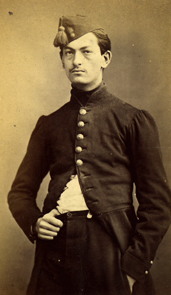
\includegraphics[width=\linewidth]{images/book3/b1-michel-levy.jpg}

{\scriptsize Michel-Lévy as a student, about 1862. Public domain.}
\end{minipage}
\end{history}

Two waves leaving a grain can be given an extra, known \omterm{def:b1:optical-mineralogy:retardation}{retardation} by an
accessory plate inserted above the section at \ang{45} to the polars. The
commonest one is cut to show the \omterm{def:b1:optical-mineralogy:interference-colour}{first-order} red, a \omterm{def:b1:optical-mineralogy:retardation}{retardation} of about
\qty{540}{nm}. If the slow vibration direction of the grain is parallel to
the slow direction of the plate, the delays add and the grain's colour rises
by about one \omterm{def:b1:optical-mineralogy:interference-colour}{order}; if it is parallel to the fast direction, they subtract and
the colour falls. A \omterm{def:b1:optical-mineralogy:interference-colour}{first-order} grey grain of \qty{100}{nm} becomes
\omterm{def:b1:optical-mineralogy:interference-colour}{second-order} blue (\qty{640}{nm}) in one orientation and \omterm{def:b1:optical-mineralogy:interference-colour}{first-order} orange
(\qty{440}{nm}) in the other; the test shows which of the grain's two
vibration directions is the slow one, a property used to identify elongated
\omterm{def:b1:rock-forming-minerals:mineral}{minerals}.

\section{Identifying minerals in thin section}

\begin{definition}[Twin, polysynthetic twinning]\label{def:b1:optical-mineralogy:twin}
A \emph{twin}\index{twin (crystal)} is an intergrowth of two or more crystals
of the same \omterm{def:b1:rock-forming-minerals:mineral}{mineral} whose lattices are related by a symmetry that the crystal
itself does not have, such as a reflection across a plane (the twin plane).
\emph{Polysynthetic twinning}\index{polysynthetic twinning} is repeated
twinning on parallel planes, which divides a crystal into thin parallel
lamellae whose orientations alternate.
\end{definition}

Between \omterm{def:b1:field-lab-methods-1:microscope}{crossed polars} the lamellae of a polysynthetic \omterm{def:b1:optical-mineralogy:twin}{twin} extinguish
alternately: half of them are dark when the other half are bright, and the
crystal looks striped. \omterm{def:b1:rock-forming-minerals:groups}{Plagioclase} almost always shows these stripes, which
distinguish it at once from quartz and from \omterm{def:b1:rock-forming-minerals:groups}{alkali feldspar}; its other
feature, low \omterm{def:b1:optical-mineralogy:relief}{relief} and \omterm{def:b1:optical-mineralogy:interference-colour}{first-order} grey to white colours, it shares with
them. The \omterm{def:b1:optical-mineralogy:extinction}{extinction angles} of the two sets of lamellae, measured either side
of the \omterm{def:b1:optical-mineralogy:twin}{twin} plane, depend on the composition of the \omterm{def:b1:rock-forming-minerals:groups}{plagioclase}, and charts
of those angles give its anorthite content.

\begin{method}[Identifying a mineral in thin section]\label{met:b1:optical-mineralogy:identify}
\begin{enumerate}
  \item In \omterm{def:b1:field-lab-methods-1:microscope}{plane-polarised light}: note whether the grain is opaque; its
        colour and \omterm{def:b1:optical-mineralogy:pleochroism}{pleochroism} (rotate the stage); its \omterm{def:b1:optical-mineralogy:relief}{relief}, and on which
        side of $1.54$ its index lies (\omterm{def:b1:optical-mineralogy:relief}{Becke line}); its shape and cleavages,
        and the angle between two cleavages.
  \item Between \omterm{def:b1:field-lab-methods-1:microscope}{crossed polars}: check whether it stays dark (isotropic, or a
        section perpendicular to an \omterm{def:b1:optical-mineralogy:optic-axis}{optic axis}); among the grains of the same
        \omterm{def:b1:rock-forming-minerals:mineral}{mineral}, find the highest \omterm{def:b1:optical-mineralogy:interference-colour}{interference colour} and read the
        \omterm{def:b1:optical-mineralogy:birefringence}{birefringence} on the \omterm{def:b1:optical-mineralogy:interference-colour}{Michel-Lévy chart} for the thickness of the
        section.
  \item Measure the \omterm{def:b1:optical-mineralogy:extinction}{extinction angle} on grains showing a cleavage or an
        elongation; look for twinning (polysynthetic stripes, simple \omterm{def:b1:optical-mineralogy:twin}{twins}).
  \item Compare with a table of optical properties
        (\cref{tab:b1:optical-mineralogy:key}) and with the \omterm{def:b1:rock-forming-minerals:mineral}{minerals} the rock
        can contain (\cref{ch:b1:rock-forming-minerals}).
\end{enumerate}
\end{method}

\begin{table}[htbp]
\centering\footnotesize
\setlength{\tabcolsep}{3pt}
% ledger: hom:quartz-optics, hom:orthoclase-optics, hom:albite-optics, hom:anorthite-optics, hom:muscovite-optics, hom:biotite-optics, hom:hornblende-optics, hom:diopside-optics, hom:forsterite-optics, hom:fayalite-optics, hom:almandine-optics, hom:calcite-optics, hom:magnetite-optics
\begin{tabular}{@{}>{\raggedright\arraybackslash}p{2.0cm}>{\raggedright\arraybackslash}p{2.6cm}>{\raggedright\arraybackslash}p{2.3cm}>{\raggedright\arraybackslash}p{1.8cm}>{\raggedright\arraybackslash}p{3.0cm}>{\raggedright\arraybackslash}p{3.8cm}@{}}
\hline
\omterm{def:b1:rock-forming-minerals:mineral}{mineral} & colour (PPL) & indices & \omterm{def:b1:optical-mineralogy:birefringence}{birefringence} & highest colour at \qty{30}{\micro m} & other features \\
\hline
quartz & colourless & 1.544--1.553 & 0.009 & \omterm{def:b1:optical-mineralogy:interference-colour}{first-order} white & no cleavage; no \omterm{def:b1:optical-mineralogy:twin}{twins} visible; \omterm{def:b1:optical-mineralogy:optic-axis}{uniaxial} \\
orthoclase & colourless, often cloudy & 1.518--1.525 & 0.005 & \omterm{def:b1:optical-mineralogy:interference-colour}{first-order} grey & negative \omterm{def:b1:optical-mineralogy:relief}{relief}; simple \omterm{def:b1:optical-mineralogy:twin}{twins} \\
\omterm{def:b1:rock-forming-minerals:groups}{plagioclase} & colourless & 1.526--1.590 & 0.008--0.013 & \omterm{def:b1:optical-mineralogy:interference-colour}{first-order} white to pale yellow & \omterm{def:b1:optical-mineralogy:twin}{polysynthetic twinning} \\
muscovite & colourless & 1.552--1.618 & 0.035--0.042 & bright second- to \omterm{def:b1:optical-mineralogy:interference-colour}{third-order} & one perfect cleavage; straight extinction \\
biotite & brown, green & 1.565--1.696 & 0.04--0.07 & masked by its own colour & strong \omterm{def:b1:optical-mineralogy:pleochroism}{pleochroism}; one perfect cleavage \\
hornblende & green, brown & 1.675--1.695 & 0.020 & \omterm{def:b1:optical-mineralogy:interference-colour}{second-order} blue & \omterm{def:b1:optical-mineralogy:pleochroism}{pleochroic}; cleavages at \ang{56}/\ang{124}; extinction \ang{15}--\ang{19} \\
diopside & colourless & 1.664--1.694 & 0.030 & \omterm{def:b1:optical-mineralogy:interference-colour}{second-order} yellow & cleavages at about \ang{87}/\ang{93}; extinction about \ang{38} \\
\omterm{def:b1:rock-forming-minerals:groups}{olivine} & colourless (Mg) to pale yellow (Fe) & 1.635--1.879 & 0.035--0.052 & end of second \omterm{def:b1:optical-mineralogy:interference-colour}{order} to third \omterm{def:b1:optical-mineralogy:interference-colour}{order} & high \omterm{def:b1:optical-mineralogy:relief}{relief}; irregular cracks, no good cleavage \\
\omterm{def:b1:rock-forming-minerals:groups}{garnet} & colourless to pale pink & 1.830 (almandine) & isotropic & black & very high \omterm{def:b1:optical-mineralogy:relief}{relief}; six- or eight-sided outlines \\
calcite & colourless & 1.486--1.658 & 0.172 & \omterm{def:b1:optical-mineralogy:interference-colour}{high-order} white & \omterm{def:b1:optical-mineralogy:relief}{relief} changes on rotation; rhombohedral cleavage \\
magnetite & opaque & --- & --- & --- & black in both lights \\
\hline
\end{tabular}
\caption{Optical properties of common rock-forming \omterm{def:b1:rock-forming-minerals:mineral}{minerals} in \omterm{def:b1:field-lab-methods-1:thin-section}{thin section}.
PPL: \omterm{def:b1:field-lab-methods-1:microscope}{plane-polarised light}. The highest colour is read on the \omterm{def:b1:optical-mineralogy:interference-colour}{Michel-Lévy
chart} at $\Delta = \qty{30000}{nm}\times\delta$.}
\label{tab:b1:optical-mineralogy:key}
\end{table}

\begin{omfigure}
\setlength{\tabcolsep}{2pt}
\begin{tabular}{cc}
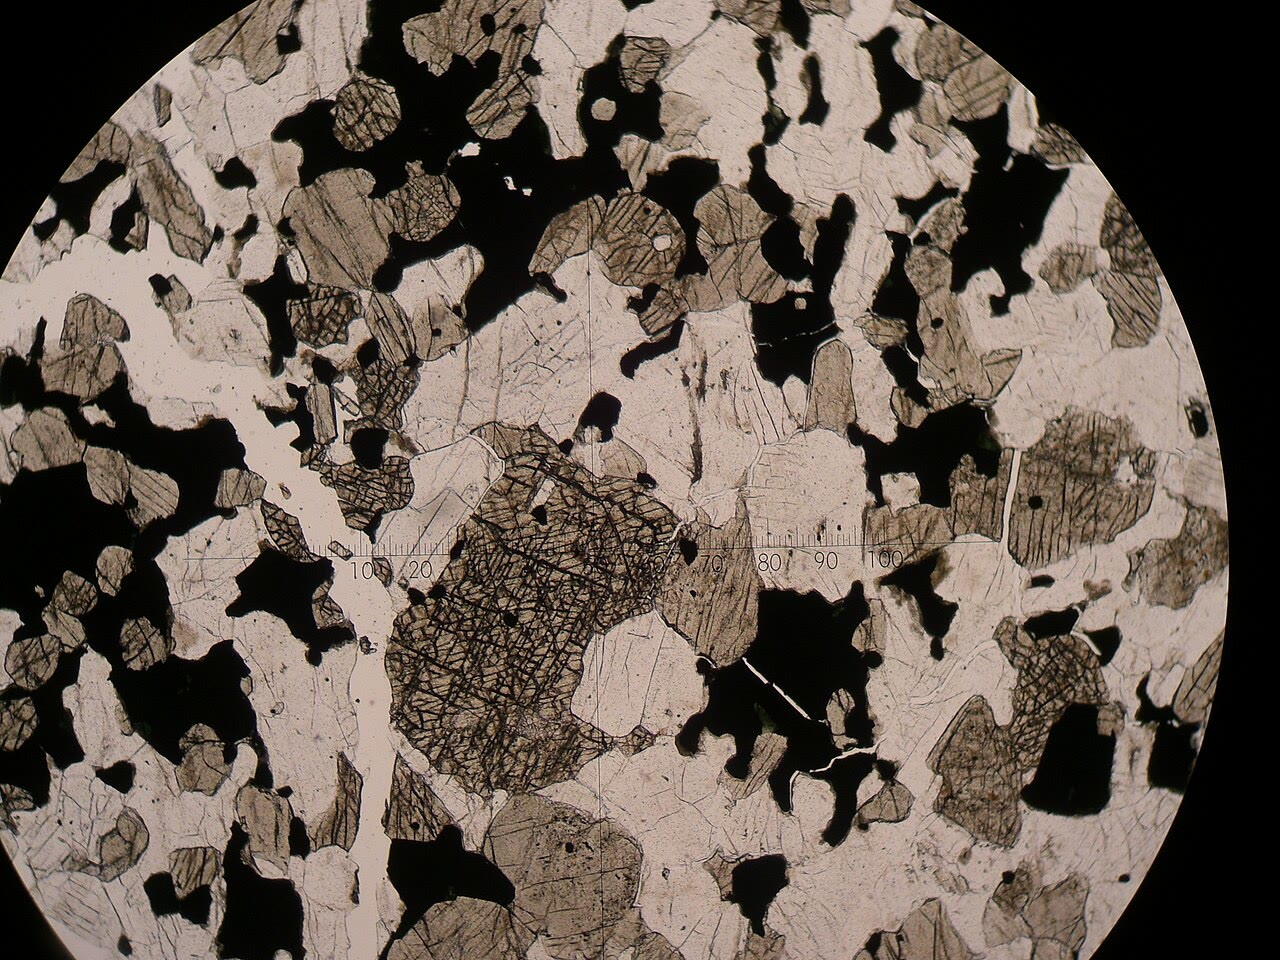
\includegraphics[width=0.485\linewidth]{images/book3/b1-gabbro-ppl.jpg} &
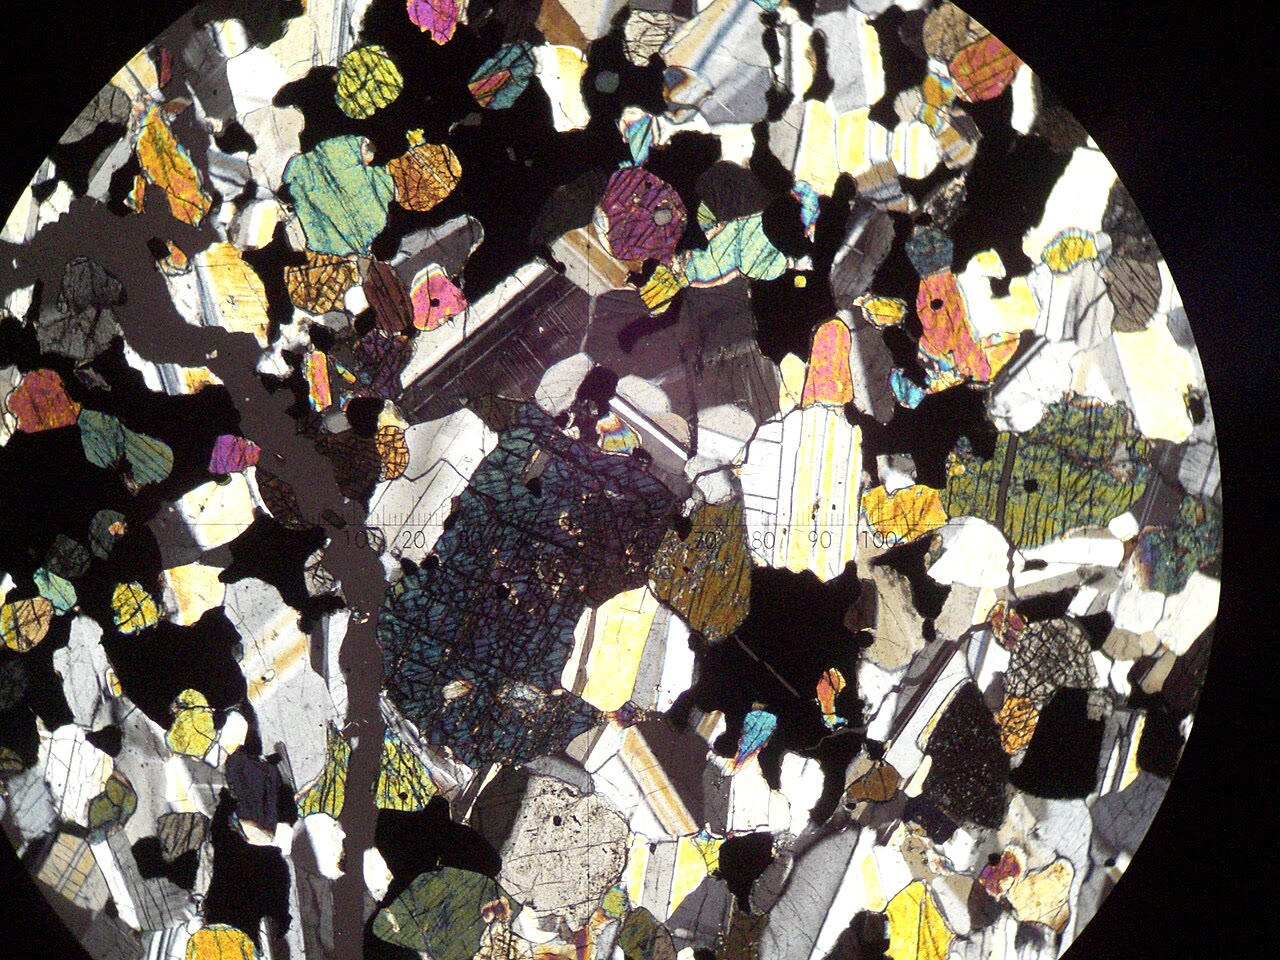
\includegraphics[width=0.485\linewidth]{images/book3/b1-gabbro-xpl.jpg} \\
{\small (a) \omterm{def:b1:field-lab-methods-1:microscope}{plane-polarised light}} & {\small (b) \omterm{def:b1:field-lab-methods-1:microscope}{crossed polars}} \\
\end{tabular}
% ledger: commons:gabbro-ppl, commons:gabbro-xpl

\medskip
{\small The same field of a gabbro in \omterm{def:b1:field-lab-methods-1:thin-section}{thin section}. In \omterm{def:b1:field-lab-methods-1:microscope}{plane-polarised light}
(a), \omterm{def:b1:rock-forming-minerals:groups}{plagioclase} is colourless with low \omterm{def:b1:optical-mineralogy:relief}{relief}, the \omterm{def:b1:rock-forming-minerals:groups}{pyroxene} and \omterm{def:b1:rock-forming-minerals:groups}{olivine}
grains are pale brown-grey with high \omterm{def:b1:optical-mineralogy:relief}{relief} and dense cracks, and the opaque
ore is black; the scale is a micrometer in the eyepiece. Between \omterm{def:b1:field-lab-methods-1:microscope}{crossed
polars} (b), the \omterm{def:b1:rock-forming-minerals:groups}{plagioclase} laths are striped by \omterm{def:b1:optical-mineralogy:twin}{polysynthetic twinning}, the
\omterm{def:b1:rock-forming-minerals:groups}{pyroxene} and \omterm{def:b1:rock-forming-minerals:groups}{olivine} grains shine in \omterm{def:b1:optical-mineralogy:interference-colour}{second-order} colours, and the ore stays
black. Photographs Chmee2, CC BY-SA 3.0 (Wikimedia Commons).}
\end{omfigure}

\begin{inthelab}[A session at the microscope]
\begin{minipage}[t]{0.55\linewidth}\vspace{0pt}
A petrologist describing a new \omterm{def:b1:field-lab-methods-1:thin-section}{thin section} works through it at low
magnification first, to see the texture and the main \omterm{def:b1:rock-forming-minerals:mineral}{minerals}, then grain by
grain. For each \omterm{def:b1:rock-forming-minerals:mineral}{mineral} she records the observations of the method above,
estimates its proportion in the field, and notes how the grains touch: which
crystallised first, which fill the spaces left, which replace others. Light
measurements are made with the stage graduated in degrees and an accessory
plate; compositions, when they matter, are measured later with a microprobe on
the same section. A teaching laboratory works the same way, one microscope per
student and a box of reference sections of known \omterm{def:b1:rock-forming-minerals:mineral}{minerals} beside it.
\end{minipage}\hfill
\begin{minipage}[t]{0.42\linewidth}\vspace{0pt}
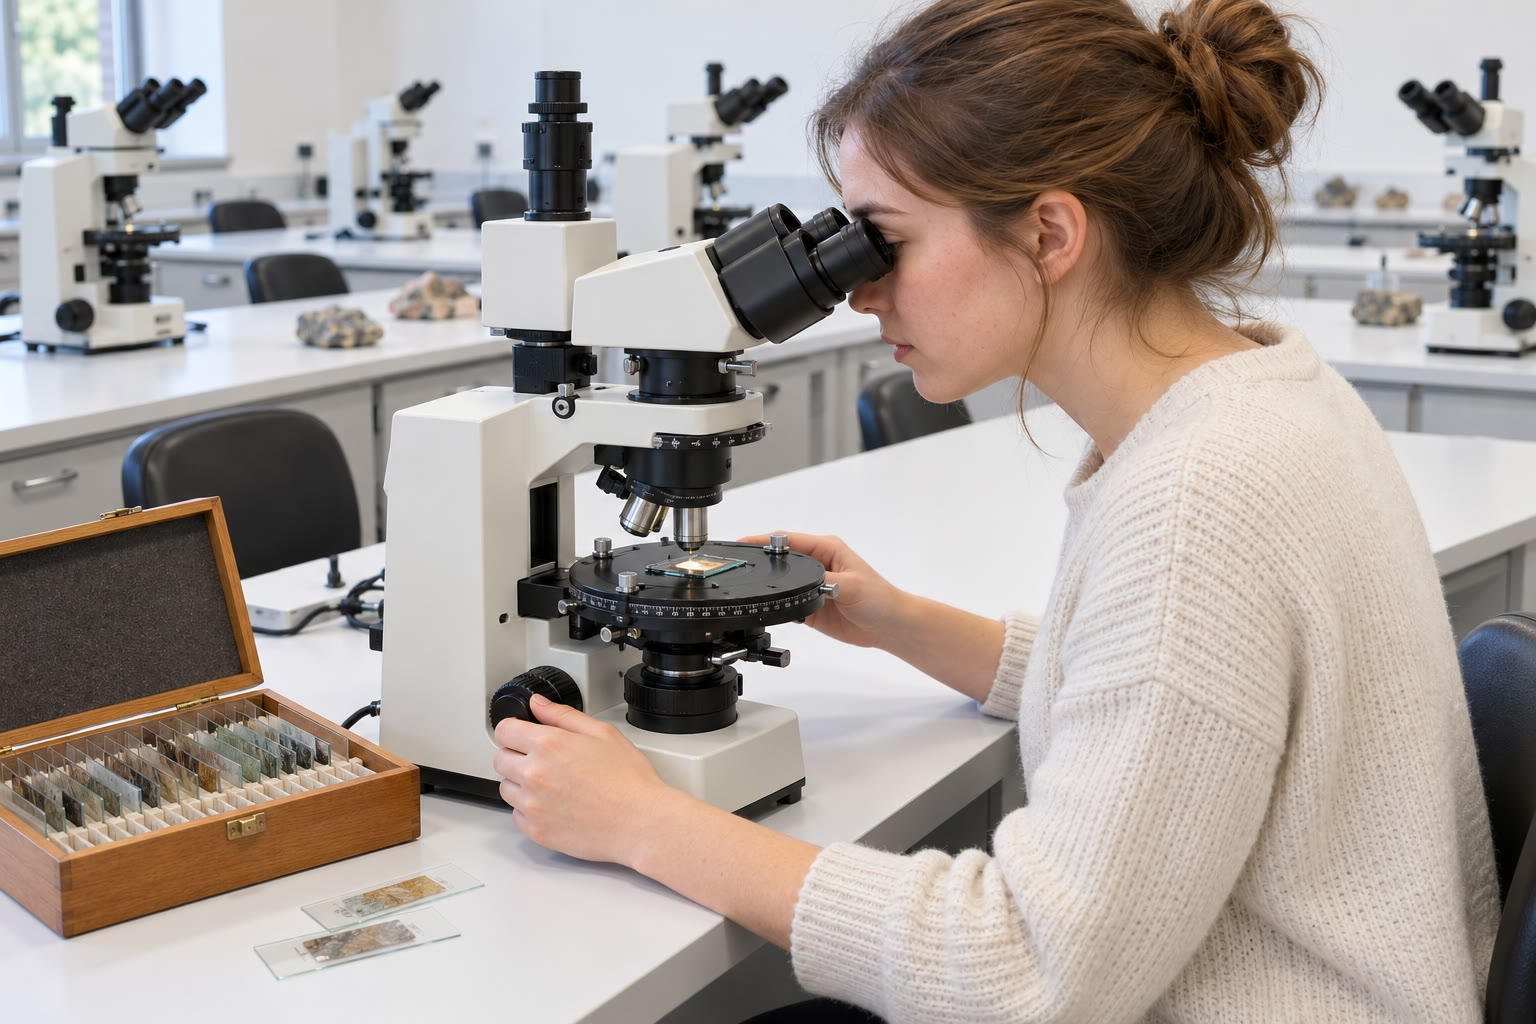
\includegraphics[width=\linewidth]{images/book3/ai/b1-microscope-student.jpg}

{\scriptsize A student at a \omterm{def:b1:field-lab-methods-1:microscope}{polarising microscope} in a teaching laboratory
(AI-generated illustration).}
\end{minipage}
\end{inthelab}

\section{Exercises}

\begin{exercise}[$\star$]\label{exo:b1:optical-mineralogy:1}
Compute the largest \omterm{def:b1:optical-mineralogy:retardation}{retardation} of quartz ($\delta = 0.009$) and of calcite
($\delta = 0.172$) in a section \qty{30}{\micro m} thick. Using the
\omterm{def:b1:optical-mineralogy:interference-colour}{Michel-Lévy chart}, describe the colour of each.
% ledger: hom:quartz-optics, hom:calcite-optics
\end{exercise}

\begin{exercise}[$\star$]\label{exo:b1:optical-mineralogy:2}
A grain is turned on the stage between \omterm{def:b1:field-lab-methods-1:microscope}{crossed polars}. Compute $I/I_0$, as a
fraction of its maximum, at $\theta = 0$, \ang{22.5}, \ang{45}, \ang{67.5} and
\ang{90} from an \omterm{def:b1:optical-mineralogy:extinction}{extinction position}.
\end{exercise}

\begin{exercise}[$\star$]\label{exo:b1:optical-mineralogy:3}
Explain why a \omterm{def:b1:rock-forming-minerals:groups}{garnet} stays black between \omterm{def:b1:field-lab-methods-1:microscope}{crossed polars} whatever the position
of the stage, and why a quartz grain may do the same. How would you tell
them apart in \omterm{def:b1:field-lab-methods-1:microscope}{plane-polarised light}?
\end{exercise}

\begin{exercise}[$\star$]\label{exo:b1:optical-mineralogy:4}
Rank by \omterm{def:b1:optical-mineralogy:relief}{relief}, in a mount of index $1.54$, orthoclase ($n$ about $1.52$),
quartz ($1.55$), forsterite ($1.65$) and almandine ($1.83$). Which has negative
\omterm{def:b1:optical-mineralogy:relief}{relief}? In which direction does its \omterm{def:b1:optical-mineralogy:relief}{Becke line} move when the focus is
raised?
% ledger: hom:orthoclase-optics, hom:quartz-optics, hom:forsterite-optics, hom:almandine-optics
\end{exercise}

\begin{exercise}[$\star\star$]\label{exo:b1:optical-mineralogy:5}
In a \qty{30}{\micro m} section, the grains of a green \omterm{def:b1:optical-mineralogy:pleochroism}{pleochroic} \omterm{def:b1:rock-forming-minerals:mineral}{mineral} with
two cleavages at \ang{56} and \ang{124} show at most a \omterm{def:b1:optical-mineralogy:interference-colour}{second-order} blue,
read on the chart as $\Delta = \qty{650}{nm}$. Compute its \omterm{def:b1:optical-mineralogy:birefringence}{birefringence} and
name the \omterm{def:b1:rock-forming-minerals:mineral}{mineral} with \cref{tab:b1:optical-mineralogy:key}.
\end{exercise}

\begin{exercise}[$\star\star$]\label{exo:b1:optical-mineralogy:6}
Using \cref{prop:b1:optical-mineralogy:relief} with $n_m = 1.54$ and
$i = \ang{30}$, compute the deviation at the edge of a quartz grain
($n = 1.553$) and of a forsterite grain ($n = 1.651$), in degrees, and the
ratio of the two. Check the second with Snell's law exactly.
\end{exercise}

\begin{exercise}[$\star\star$]\label{exo:b1:optical-mineralogy:7}
A \omterm{def:b1:optical-mineralogy:interference-colour}{first-order} red plate has $\Delta = \qty{540}{nm}$. A quartz grain of
$\Delta = \qty{270}{nm}$ is placed at \ang{45} with the plate inserted. What
are the two possible total \omterm{def:b1:optical-mineralogy:retardation}{retardations}, and the colours they give on the
chart? Which orientation puts the two slow directions parallel?
\end{exercise}

\begin{exercise}[$\star\star$]\label{exo:b1:optical-mineralogy:8}
At its tapering edge, a grain of fayalite ($\delta = 0.052$) thins from
\qty{30}{\micro m} to zero. How many red-violet tints, which end the \omterm{def:b1:optical-mineralogy:interference-colour}{orders}
at 542, 1074 and \qty{1605}{nm}, appear as coloured fringes between the edge
and the full-thickness part of the grain?
% ledger: hom:fayalite-optics
\end{exercise}

\begin{exercise}[$\star\star$]\label{exo:b1:optical-mineralogy:9}
On several elongated grains with one good cleavage, a geologist measures
\omterm{def:b1:optical-mineralogy:extinction}{extinction angles} of \ang{0}, \ang{21}, \ang{36} and \ang{37} between the
cleavage trace and the slow vibration direction. Why do the values differ?
Is the \omterm{def:b1:rock-forming-minerals:mineral}{mineral} more likely diopside or hornblende?
% ledger: hom:diopside-optics, hom:hornblende-optics
\end{exercise}

\begin{exercise}[$\star\star\star$]\label{exo:b1:optical-mineralogy:10}
Redo the proof of \cref{thm:b1:optical-mineralogy:intensity} with the
analyser parallel to the polariser, and show that
$I_\parallel = I_0\bigl(1 - \sin^2 2\theta\sin^2(\pi\Delta/\lambda)\bigr)$.
What colour does a grain of $\Delta = \qty{550}{nm}$ show at \ang{45}
between parallel polars?
\end{exercise}

\begin{exercise}[$\star\star\star$]\label{exo:b1:optical-mineralogy:11}
For a calcite grain with $\Delta = \qty{5000}{nm}$, the factor
$\sin^2(\pi\Delta/\lambda)$ vanishes whenever $\Delta/\lambda$ is a whole
number. (a) How many times does it vanish between \num{400} and
\qty{700}{nm}? (b) Show that near $\lambda = \qty{550}{nm}$ two successive
zeros are about $\lambda^2/\Delta$ apart, and compute it. (c) Explain why the
grain looks nearly white.
\end{exercise}

\begin{exercise}[$\star\star\star$]\label{exo:b1:optical-mineralogy:12}
Show that, averaged over a full turn of the stage, a grain between \omterm{def:b1:field-lab-methods-1:microscope}{crossed
polars} passes $\frac12 I_0\sin^2(\pi\Delta/\lambda)$. A geologist estimates
\omterm{def:b1:optical-mineralogy:birefringence}{birefringences} from the highest colour of each \omterm{def:b1:rock-forming-minerals:mineral}{mineral}, assuming
\qty{30}{\micro m}, in a section that is in fact \qty{25}{\micro m} thick. By
what factor are all her values wrong, and in which direction?
\end{exercise}

\section{Problem: Identifying the minerals of an unknown thin section}

\begin{problem}[{Weekend problem --- observing relief, pleochroism and
interference colours, measuring the thickness of a section with quartz, and
naming its minerals}]
\label{pb:b1:optical-mineralogy:1}
% values: calc/ch08.py; optical data: ledger hom:*-optics
% ledger: hom:quartz-optics, hom:diopside-optics, hom:forsterite-optics, hom:albite-optics, hom:anorthite-optics, hom:hornblende-optics, hom:biotite-optics
A \omterm{def:b1:field-lab-methods-1:thin-section}{thin section} of an unknown igneous rock, mounted in a resin of index
$1.540$, is said to be \qty{30}{\micro m} thick. It contains five \omterm{def:b1:rock-forming-minerals:mineral}{minerals},
labelled A to E. Use the table of optical properties of the chapter, the
\omterm{def:b1:optical-mineralogy:interference-colour}{Michel-Lévy chart}, and the following values: quartz $n_\omega = 1.544$,
$n_\varepsilon = 1.553$; diopside $n_\alpha = 1.664$, $n_\beta = 1.672$,
$n_\gamma = 1.694$.

\medskip
\noindent\textbf{Part I --- Plane-polarised light.}
\begin{enumerate}
  \item \omterm{def:b1:rock-forming-minerals:mineral}{Mineral} A is colourless, with grain boundaries hard to see. \omterm{def:b1:rock-forming-minerals:mineral}{Mineral} B
        is colourless, with strong dark rims and two cleavages meeting at
        about \ang{87}. Which has the higher \omterm{def:b1:optical-mineralogy:relief}{relief}?
  \item For A, taken as quartz, and B, taken as diopside, compute
        $|n - n_m|$ using the mean of the principal indices of each.
  \item Using \cref{prop:b1:optical-mineralogy:relief}, compute the ratio of
        the deviations at their edges for the same inclination of the boundary.
  \item On raising the focus, the \omterm{def:b1:optical-mineralogy:relief}{Becke line} of B moves into the grain. What
        does this show?
  \item \omterm{def:b1:rock-forming-minerals:mineral}{Mineral} C turns from pale yellow to dark brown as the stage rotates,
        darkest when its single cleavage lies along the polariser. Name the
        property and the \omterm{def:b1:rock-forming-minerals:mineral}{mineral}.
  \item \omterm{def:b1:rock-forming-minerals:mineral}{Mineral} D is colourless, of low \omterm{def:b1:optical-mineralogy:relief}{relief}, in long laths; E is green to
        yellow and \omterm{def:b1:optical-mineralogy:pleochroism}{pleochroic}, with two cleavages at \ang{124}. What does the
        angle suggest for E?
\end{enumerate}

\medskip
\noindent\textbf{Part II --- The thickness of the section.}
\begin{enumerate}[resume]
  \item What is the largest \omterm{def:b1:optical-mineralogy:retardation}{retardation} of quartz in a section of exactly
        \qty{30}{\micro m}? What colour is it?
  \item Why must the largest \omterm{def:b1:optical-mineralogy:retardation}{retardation} be sought among many grains of A,
        rather than measured on any one of them?
  \item The highest colour shown by the grains of A is a \omterm{def:b1:optical-mineralogy:interference-colour}{first-order} pale
        yellow; a quartz-wedge comparator gives its \omterm{def:b1:optical-mineralogy:retardation}{retardation} as
        \qty{342}{nm}. Compute the real thickness of the section.
  \item By how many per cent is the section thicker than it should be?
  \item At $\lambda = \qty{550}{nm}$ and \ang{45} from extinction, compute
        $I/I_0$ for this quartz grain, and for the same grain in a section of
        \qty{30}{\micro m}.
  \item Compute the range of \omterm{def:b1:optical-mineralogy:retardation}{retardations} of D, taken as \omterm{def:b1:rock-forming-minerals:groups}{plagioclase}
        ($\delta = 0.008$ to $0.013$), in this section, and say whether its
        colours remain in the first \omterm{def:b1:optical-mineralogy:interference-colour}{order}.
\end{enumerate}

\medskip
\noindent\textbf{Part III --- The birefringence of B.}
\begin{enumerate}[resume]
  \item The highest colour of B is a blue read as $\Delta = \qty{1140}{nm}$.
        In which \omterm{def:b1:optical-mineralogy:interference-colour}{order} is it?
  \item Compute the \omterm{def:b1:optical-mineralogy:birefringence}{birefringence} of B with the thickness found in
        question 9.
  \item What \omterm{def:b1:optical-mineralogy:birefringence}{birefringence} would one have found by assuming
        \qty{30}{\micro m}? Which colourless \omterm{def:b1:rock-forming-minerals:mineral}{mineral} of high \omterm{def:b1:optical-mineralogy:relief}{relief} would
        that have suggested, and why is it out of place in a rock with quartz
        (consider \ce{Mg2SiO4 + SiO2 -> 2 MgSiO3})?
  \item Compare the result of question 14 with the table, together with the
        \omterm{def:b1:optical-mineralogy:relief}{relief} and the cleavages of B, and conclude.
  \item What colour would B show at most in a correct \qty{30}{\micro m}
        section?
  \item The section is ground down to \qty{30}{\micro m}. By how much must it
        be thinned, and what is then the highest colour of quartz?
\end{enumerate}

\medskip
\noindent\textbf{Part IV --- Extinction and twinning.}
\begin{enumerate}[resume]
  \item The laths of D are divided into parallel stripes that extinguish
        alternately. Name the feature and the \omterm{def:b1:rock-forming-minerals:mineral}{mineral}.
  \item The stripes of one lath extinguish at \ang{27} and \ang{28} either side
        of the \omterm{def:b1:optical-mineralogy:twin}{twin} plane. What do such angles, measured on many laths, give
        when compared with published charts?
  \item The highest \omterm{def:b1:optical-mineralogy:extinction}{extinction angle} between the cleavages of E and its slow
        direction is \ang{17}. Name E.
  \item Compute the largest \omterm{def:b1:optical-mineralogy:retardation}{retardation} of E in this section and the colour
        it shows.
  \item A grain of B stays dark during a full rotation. Explain how it can be
        the same \omterm{def:b1:rock-forming-minerals:mineral}{mineral} as the bright grains of B.
  \item List the \omterm{def:b1:rock-forming-minerals:mineral}{minerals} A to E, and say what kind of rock they make.
  \item What is the real thickness of the section, in micrometres?
\end{enumerate}
\end{problem}
